% Latex template: https://github.com/mqTeXUsers/Macquarie-University-Beamer-Theme

% Slide Masters:

% Title
% Text
% 2 column
% Full-image
% Bibliography
% Closing
 
\documentclass[aspectratio=1610, 11pt]{beamer} % Aspect ratio
% https://tex.stackexchange.com/a/14339/5483 
% Possible values: 1610, 169, 149, 54, 43 and 32.
% 169 = 16:9

\PassOptionsToPackage{table}{xcolor}    %https://tex.stackexchange.com/a/5365/5483

\usetheme{macquarie}
\usepackage{multicol} % https://tex.stackexchange.com/a/396018/5483
\usepackage{xurl}
\usepackage[british]{babel}       % Set language
% \usepackage[utf8x]{inputenc}      % Set encoding
\usepackage{colortbl}
\mode<presentation>           % Set options
{
  \usetheme{default}          % Set theme
  \usecolortheme{default}         % Set colors
  \usefonttheme{default}          % Set font theme
  \setbeamertemplate{caption}[numbered] % Set caption to be numbered
}

% Uncomment this to have the outline at the beginning of each section highlighted.
%\AtBeginSection[]
%{
%  \begin{frame}{Outline}
%    \tableofcontents[currentsection]
%  \end{frame}
%}

\usepackage{graphicx}         % For including figures
\usepackage{booktabs}         % For table rules
\usepackage{hyperref}         % For cross-referencing


%\usepackage{enumitem} % https://tex.stackexchange.com/a/2292/5483
\usepackage[shortlabels]{enumitem}

%https://tex.stackexchange.com/a/371844/5483
\setbeamerfont{bibliography entry author}{size=\tiny}
\setbeamerfont{bibliography entry title}{size=\tiny}
\setbeamerfont{bibliography entry location}{size=\tiny}
\setbeamerfont{bibliography entry note}{size=\tiny}
\setbeamerfont{bibliography item}{size=\tiny}

%https://tex.stackexchange.com/q/333587/5483
%TODO SHAWN REPLACE OSF URL
%\setbeamertemplate{footline}{\strut~\texttt{https://github.com/MQ-FOAR705/MQ-FOAR705-Week1}\hfill\insertframenumber~/~\inserttotalframenumber\strut~~~}

\title{FOAR705 Week 6} % Presentation title
\author{Brian Ballsun-Stanton | Shawn A Ross | Kathryn Elliot}               % Presentation author
\institute{Faculty of Arts}         % Author affiliation
\date{Friday 23 August 2019}                 % Today's date  
\begin{document}

% Title page
% This page includes the informations defined earlier including title, author/s, affiliation/s and the date
% \begin{frame}[noframenumbering]

\maketitle

  
% \end{frame}

\begin{frame}{Today's Plan}
  \tableofcontents
\end{frame}

\section{Data Carpentry}
\begin{frame}{Data Carpentry}

See lesson at: https://datacarpentry.org/openrefine-socialsci/

\end{frame}
\section{Proof of Concept Design Assignment}
\begin{frame}{Assignment overview}

We know \textit{what} we want to do. We know \textit{how} we want to do it. The remainder of the semester will be building, testing, documenting, and presenting your proof of concept. Besides the learning journal (due week 8) all other graded things are due at the end of semester.

Internal due dates:

\begin{description}
\item [Week 7] Proof of Concept - Design 
\item [Week 9] Proof of Concept - Components work
\item [Week 11] Proof of Concept - Components Linked
\end{description}

Graded: 
\begin{description}
\item [Week 13] Proof of Concept - Minimal Viable Product delivered
\end{description}
\end{frame}

\begin{frame}{Making your Design}

\begin{itemize}[label=\textbullet]
    \item Create User Stories
    \begin{itemize}[label=\textbullet]
        \item Each story has the story itself
        \item Acceptance Criteria
    \end{itemize}
    \item Categorise themes and identify prerequisites
    \item Load into project management system
    \item Share for feedback from colleagues
    \item Plan Quality Assurance (if you're aiming for HD)
    \item Sanity check and submit
\end{itemize}
    
\end{frame}

\begin{frame}{Anatomy of a User Story}

{\huge As a [role], I want [goal] so that [reason].}

\begin{figure}
    \centering
    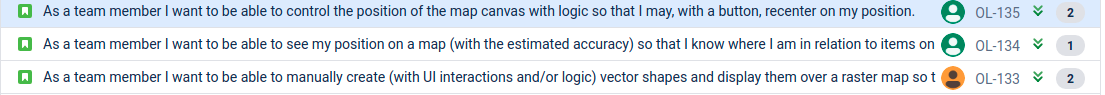
\includegraphics[width=\textwidth]{figures/userstories.png}
    \caption{User stories from 2012 when we were developing FAIMS.}
    \label{fig:userstory}
\end{figure}

Example: As a \textbf{student}, I want my \textbf{typesetting software to generate my bibliography}, so that I don’t have \textbf{to double check in text citations against my bibliography}.

It is OK to have additional description (hidden away with a click or equivalent) so that what you mean is clear to future-you. This user story is like a commit summary: short and pithy. Click through for the multi-line discussion if necessary.
\end{frame}

\begin{frame}{Acceptance Criteria}
A step by step decomposition of each action needed to make the feature described by the user story work. Differentiates between the story being completed or needing more work. Makes sure you don't skip steps.
\begin{figure}
    \centering
    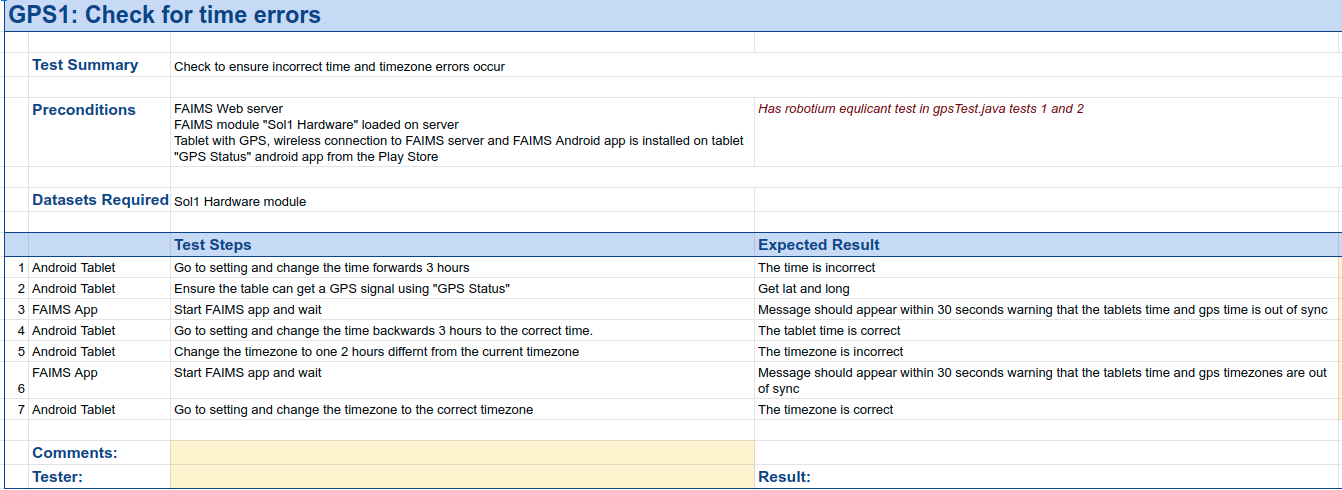
\includegraphics[width=\textwidth]{figures/acceptance.png}
    \caption{Acceptance Criteria for an update we did in 2016}
    \label{fig:my_label}
\end{figure}

If your criteria has more than 4-8 specific steps, your user story might be too broad. 
\end{frame}

\begin{frame}{Acceptance Criteria Example}

As a student, I should be able to: 
\begin{enumerate}[1.]
    \item Supply a bibliography database to the program
    \item Choose an in-text citation from the sources in the database
    \item Choose the bibliographic standard
    \item Cause the program to generate a bibliography and correct in-text citation based on the chosen citation and standard
\end{enumerate}

You can also articulate expected results if it's not immediately obvious. 

\end{frame}
\begin{frame}{User story Exercise}

For the next (half the remaining time till 3:30), work in groups of 2-3. Preferably with folk doing a similar activity or with your neighbours.

Each person in the group should:
\begin{itemize}[\textbullet]
    \item Provide a one minute summary of their desired goal (scope)
    \item One minute talk about one tool they've chosen to use.
\end{itemize}
Then, everyone should, for their own proof of concept:
\begin{itemize}[\textbullet]
    \item Create a user story for a feature they need to implement
    \item Create acceptance criteria
    \end{itemize}

Then, each group member should try to figure out if they could (with knowledge of the tool assumed) implement each others' user story to satisfy the acceptance criteria. 

\end{frame}
\section{Minute cards!}
\begin{frame}{Feedback time}

On your green sticky, write one thing we did well today.

On your red sticky, write one thing we could improve upon for next time. Be specific. 

\end{frame}

\section{Guest Lecture}
\begin{frame}{Ross Burns}

{\bf Bringing it all together—integrated sources for crunching data across disciplines, sources and regions.}

Use of Filemaker, Google Earth, Adobe Lightroom and other software to monitor sites and buildings across the Middle East, especially in areas of conflict. The aim is to take a region-wide look at the damage across all periods for which we have physical remains and in all political environments. This has produced an integrated database compiled over the last twenty years of detailed information (in the form of images, historical summaries of sites/buildings, relevant epigraphical and bibliographical sources, plans and maps from my own and other published sources) allowing an instant readout or statistical overview to inform further study, breaking down the barriers inherent in more specialised (region- or period-specific) sources.
    
\end{frame}

\section{References}

\begin{multicols}{2}[]
\bibliography{references}
\bibliographystyle{apalike}
\end{multicols}


% \begin{frame}[allowframebreaks]{References}
  
%   \bibliography{references}
%   \bibliographystyle{apalike}
% \end{frame}


\begin{frame}{Thank you!}

% This presentation is available at:
% \texttt{https://osf.io/...}

Source code for this presentation is available at: \url{https://github.com/MQ-FOAR705/MQ-FOAR705-Week3}

This work is licensed under a Creative Commons Attribution 4.0 International License.

\end{frame}



\end{document}